%% -*- coding: utf-8 -*-
\documentclass{article}
% Outline for statistics tutorial
% Hal Canaray and Cory Quammen
\usepackage{graphicx}
\usepackage{utfsymb}
\begin{document}

\begin{center}
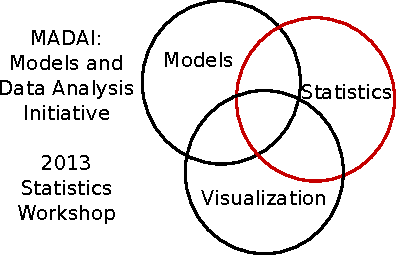
\includegraphics{figures/MADAI_2013_Stats_Workshop.pdf}
\end{center}

\section{Statistics background}

\subsection{Basic concepts}

We have a model and we're trying to find parameters for it that best
explain some observed phenomena.

\begin{itemize}

\item Model — a conceptual model of a physical process.  It exists as
  a procedure that takes in parameters and returns a set of
  outputs and potentially uncertainty about those outputs. FIXME Examples
 
\item Observables — a set of field measurements that can be compared
  against a model's outputs. FIXME Examples

\item Output Space — The set of all possible outputs of the model,
  which are intended to be compared to observables.

\item Model Outputs — a point in output space, or a point in output
  space together wuith uncertainty.

\item Model Parameters — any of the modifiable inputs to the
  model. FIXME Examples

\item Parameter Space — the set of all possible values for each of the
  parameters

\item Ground Truth — a point in parameter space that represents how
  the physical process actually works.

\item Likelihood — Given a model and set of observables, this is the
  probability of a given set of parameter values.

\item Prior Likelihood — FIXME

\newpage

\[ P = \textrm{parameter space} ⊂ ℝ^p \]
\[ T = \textrm{output space} ⊂ ℝ^t \]
\[ M: P → T \]
\[ Y_f = \textrm{distribution of field measurements} ⊂ T\]
\[ y = M(x) \]
\[
ℒ ∝ \textrm{exp}\left({-\frac{1}{2}\big(E[Y]-E[Y_f]\big)^T \big(Σ[Y]+Σ[Y_f]\big)^{-1} \big(E[Y]-E[Y_f]\big)}\right)
\]

\end{itemize}

\begin{center}
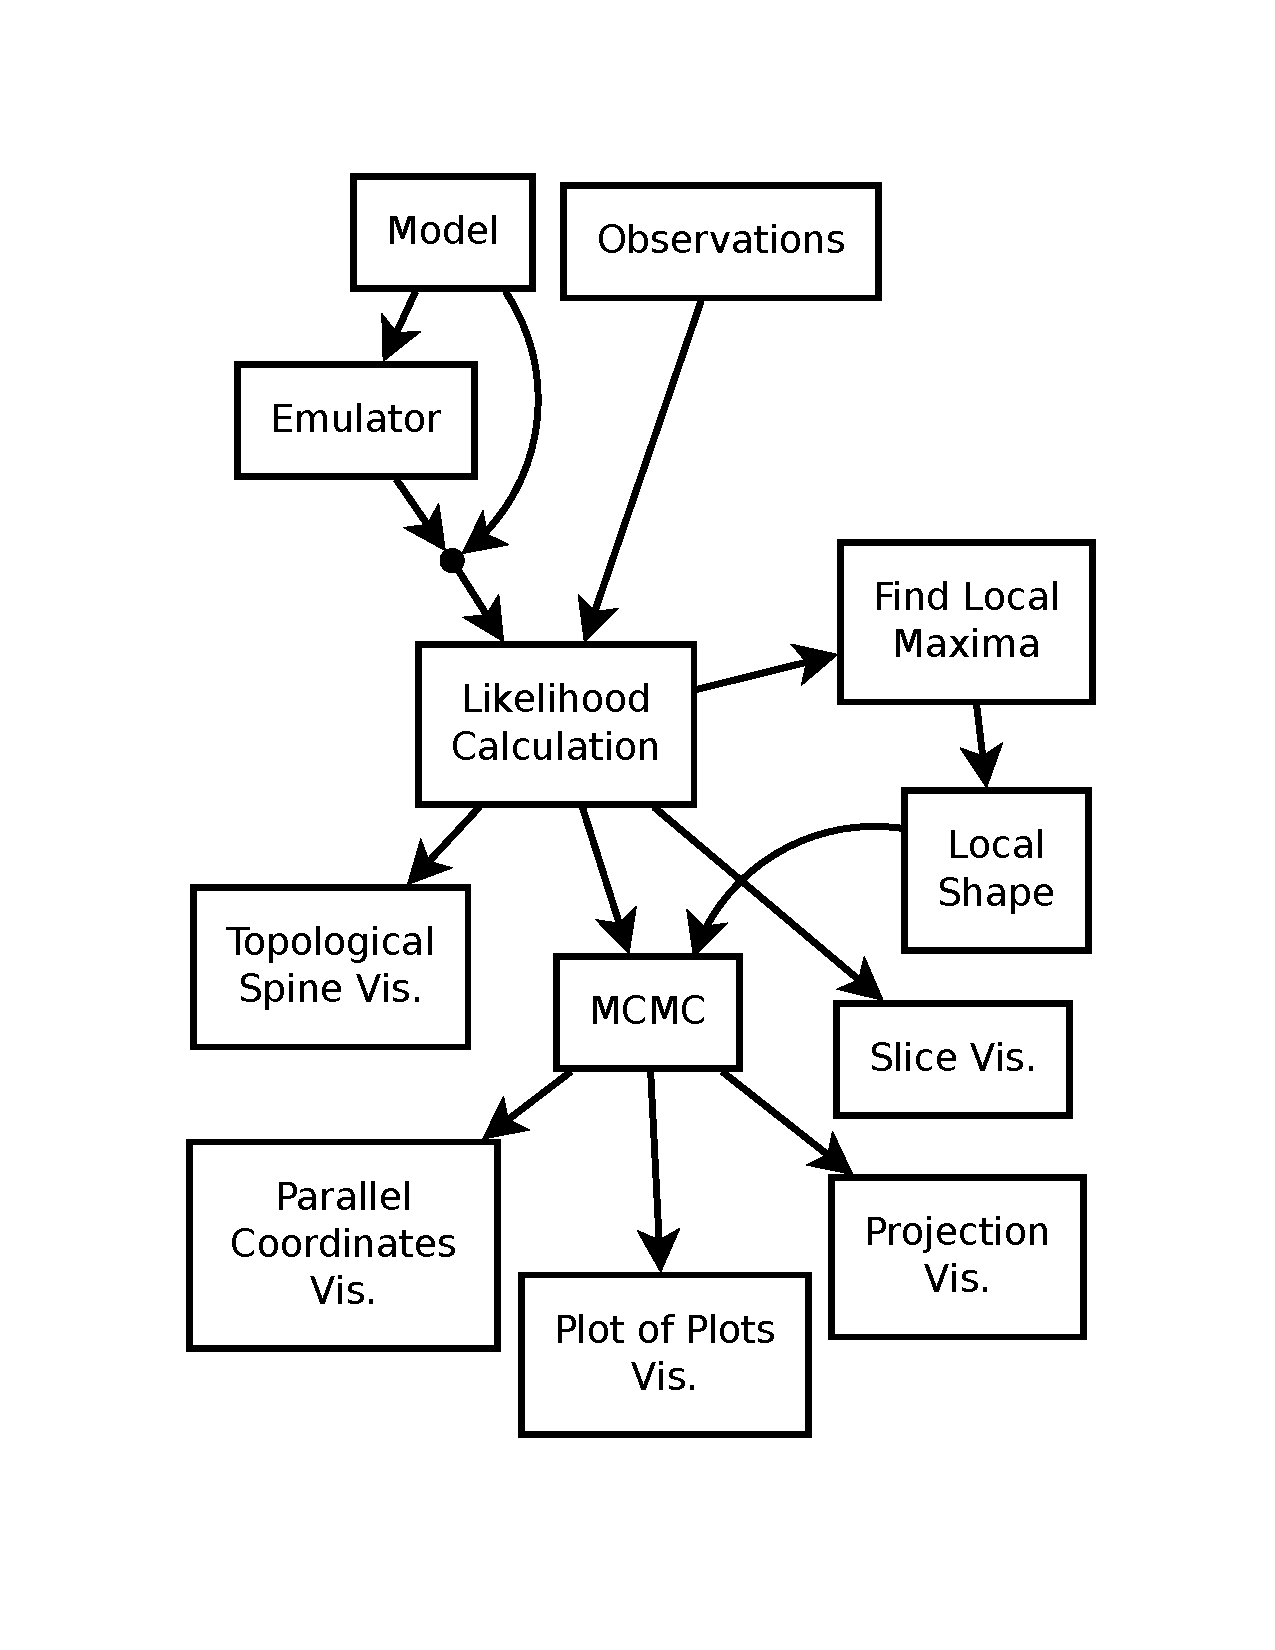
\includegraphics[width=3in]{figures/MADAI_Stats_and_Vis.pdf}
\end{center}


\subsubsection{Probability and statistics review}

Touch on terms.

Probability, expectation, distribution, joint distribution, variance,
covariance

\subsubsection{Joint implausbility}

\section{Gaussian process emulator}

\subsection{Background}

See Chris Coleman-Smith's presentation at the June 2012 MADAI meeting on this

\begin{itemize}

\item What it does?

\item Why use it instead of interpolation?

\item How to use it?

\end{itemize}

This section taken from MADAIEmulator/README

A project to implement scalar Gaussian process regression with a
variety of covariance functions with an optional (up to 3rd order)
linear regression prior mean. Maximum likelihood hyper-parameters can
be estimated to parametrize a given set of training data. For a given
model (estimated hyperparams and training data set) the posterior mean
and variance can be sampled at arbitrary locations in the parameter
space.

The model parameter space can take any dimension (within limits of the
optimizer), output must be scalar.

Gaussian Process regression is a supervised learning method, a
representative set of samples of a model's output can be used to build
a predictive distribution for the output at untried locations in the
models parameter space. This code base has been developed to apply
this process to the output of complex computer codes.

Suppose we have a model $Y_m(u)$ which produces scalar output as a
function of some set of input parameters $u$. A design is a set of
points $D = \{u_1, …, u_n\}$ in the $u$ space at which we will evaluate
the model. A set of training outputs $Y_t = \{Y_m(u_1), …, Y_m(u_n)\}$ is
produced by evaluating the model at each location in $D$. The sets $D$ and
$Y_t$ are then sufficient to 'train' a GP regression model or Emulator
to produce predictions at some new locations $u*$.

The training process conditions a Gaussian Process prior on the set
$\{Y_t, D\}$ such that functions drawn from the ensuing posterior will
always pass through the training locations. A Gaussian Process (GP) is
a stochastic process for which any finite set of samples have a multi
variate normal distribution. In essence we force the Gaussian Process
to always generate functions which interpolate our data set.

The GP is specified in terms of a prior mean, usually chosen to be
zero or given by a simple regression model of the training data, and a
covariance function over the parameter space. The covariance function
specifies the correlation between pairs of parameter values $u_i$,
$u_j$. A power exponential form, with a nugget, is the default.

\[C(u_i, u_j) = θ_0 \textrm{~exp}\big(-\frac{1}{2} ( u_i - u_j)^2 / θ_l^2\big) + θ_1. \]

The covariance function itself is controlled by a set of
hyper-parameters $θ_i$, these act as characteristic length scales in
the parameter space and are a-priori unknown. The training process
consists of estimating the 'best' set of length scales for the given
model data set. This estimation process is done through numerical
maximization of the posterior hyper parameter likelihood, a fully
Bayesian treatment is also possible.

Once the GP has been conditioned, and a best set of hyper parameters
$Θ$ has been obtained, we have a posterior predictive distribution
for the model output at a new location $u*$:

\[P(Y_m(u*) | Y_t, D, Θ) = \textrm{MVN}(m(u*), \textrm{cov}(u*)), \]

where the posterior mean and covariance are (for a zero prior mean)

\[m(u*) = C(u*,D)^t  C(D,D)^{-1} Y_t\]
\[cov(u*) = C(u*,u*) - C(u*,D)^t C(D,D)^{-1} C(u*,D).\]

Here $C(D,D)$ represents the matrix formed by evaluating the covariance
function $C(u_i, u_j)$ at each of the locations in $D$, the vector
$C(u*,D)$ =  $\{C(u*, u_1)$,$C(u*, u_2), …, $$C(u*, u_n)\}$ is the correlation
between each location in the design set and the new point.

These equations have a relatively straightforward interpretation. The
prior mean (0) is modified by the covariance structure deduced from
the data $C(u*,Y_t)^t C(D,D)^{-1} Y_t$, at $u* = u_i$ where $u_i$ is in $D$,
we can see that $m(u_i) = 0$. The prior covariance at $u*, C(u*,u*)$ is
somewhat reduced by the training set $C(u*,Y_t)^t C(D,D)^{-1}
C(u*,Y_t)$ and again at $u*=u_i$ for $u_i$ in $D$ we reduce to $\textrm{cov}(u_i) =
0$. As such we have constructed an interpolating function.

It is important to note that unlike some other data
interpolation/extrapolation methods we end up with a probability
distribution for the value of our model at an untried location, as it
is normal the mean and covariance are sufficient to describe the
distribution. These can be obtained by the emulate\_at\_point or
emulate\_at\_list functions.

It is straightforward to draw samples from the predictive
distribution, although care must be taken to expand the above
equations correctly for a set of m observation locations
$U* = {u*_1, ... u*_m}$.

For more information see the documentation, the website
http://www.gaussianprocess.org and the invaluable book "Gaussian
processes for machine learning".

\subsection{Training an emulator}

\subsubsection{What is a nugget?}

\subsubsection{Inputs}

\begin{itemize}

\item Set regression order - this subtracts a broad trend in the data to make the training better behaved

\item Pick a covariance function - this is a kernel that determines the weights of nearby training data on an output

\item PCA variance (0.0 - 1.0) - how much of the variance do you want to explain?

\end{itemize}

\subsection{Verify emulator}

Feed training points back into emulator. Results won't be identical, but should be close. Jittering parameter-space position should give you similar values.

\section{Markov Chain Monte Carlo}

\subsection{Background}

\subsection{Algorithm we use}

Metropolis-Hastings

\subsection{Burn-in}

\subsection{Post burn-in}



\section{Software session}

\subsection{Download code}

\subsubsection{MADAI Workbench}

\subsubsection{Emulator}

Set up environment for running it

\subsubsection{Data}

\begin{itemize}

\item One die example data in format useful for training. Question: How long is this going to take?

\item Two die example

\end{itemize}

\end{document}
